\documentclass[12pt,letterpaper]{article}
\usepackage[utf8]{inputenc}
\usepackage[T1]{fontenc}
\usepackage[spanish,es-noshorthands,es-tabla]{babel}
\usepackage{newtxtext,newtxmath}
\usepackage[margin=2.54cm]{geometry}
\usepackage{array,setspace,graphicx,booktabs,amsmath,tikz,float,caption}
\usepackage{algorithm,algpseudocode}
\usepackage[hidelinks]{hyperref}
\usepackage{xurl}
\usetikzlibrary{positioning}
\onehalfspacing
\setlength{\parindent}{1.27cm}
\floatname{algorithm}{Algoritmo}
\algrenewcommand\algorithmicfunction{\textbf{función}}
\algrenewcommand\algorithmicfor{\textbf{para}}
\algrenewcommand\algorithmicdo{\textbf{hacer}}
\algrenewcommand\algorithmicif{\textbf{si}}
\algrenewcommand\algorithmicthen{\textbf{entonces}}
\algrenewcommand\algorithmicreturn{\textbf{devolver}}
\algrenewcommand\algorithmicwhile{\textbf{mientras}}

\begin{document}

\begin{titlepage}
\centering
\vspace*{2cm}
{\Large\bfseries BusQuilla: modelación de la red de buses de Barranquilla como un grafo ponderado para estimar tiempos de llegada y descubrir rutas alternativas\par}
\vspace{2cm}
Camilo Cruz González\par
Nicolás Montenegro Ríos\par
Gustavo Parody Cifuentes\par
Josué Salas Mercado\par
\vspace{1cm}
Departamento de Matemáticas y Estadística, Universidad del Norte\par
\vspace{0.5cm}
Matemáticas Discretas (MAT 4021)\par
Profesor: MSc Iván Gómez\par
\vspace{0.5cm}
15 de noviembre de 2026\par
\vfill
\end{titlepage}

\section*{Resumen}
En el Área Metropolitana de Barranquilla viven más de 2,2 millones de personas y cerca de la mitad de quienes se desplazan a diario dependen del bus tradicional o de Transmetro. Sin embargo, el usuario promedio no sabe en qué momento pasará el próximo bus ni conoce todas las rutas que podrían llevarlo a su destino: suele usar siempre la misma ruta y esperar en el paradero sin información. En este trabajo se modela la red de transporte público como un grafo ponderado no dirigido $G=(V,E,w)$, en el que los vértices son paraderos, las aristas representan tramos recorridos en bus o caminatas de transbordo, y los pesos son tiempos en minutos. Con datos reales de 41 rutas obtenidas de OpenStreetMap (1\,815 puntos de parada y 17\,113 aristas) se construyó \textit{BusQuilla}, una aplicación web que (i) simula en vivo la posición de los buses y sus conductores, (ii) calcula cuánto tarda el próximo bus de cada ruta en llegar a la zona elegida por el usuario y (iii) encuentra el viaje más rápido entre dos puntos mediante el algoritmo de Dijkstra, incluyendo transbordos. En una muestra de 300 viajes aleatorios, el 60\,\% de los viajes en los que conviene el bus requieren al menos un transbordo, lo que confirma que el problema no es solo de espera sino de desconocimiento de la red. Los viajes recomendados toman en promedio 32,9 minutos frente a 52,6 minutos caminando. Se discuten además las propiedades estructurales de la red (grados, conectividad y densidad) y las limitaciones del modelo.

\noindent\textit{Palabras clave:} teoría de grafos, camino más corto, algoritmo de Dijkstra, transporte público, Barranquilla, información en tiempo real.

\section{Introducción}

\subsection{El problema}
Cualquier barranquillero conoce la escena: una persona parada en una esquina, bajo el sol de mediodía, mirando hacia el fondo de la calle sin saber si el bus viene en dos minutos o en veinte. A su lado pasan buses de otras rutas que también la habrían dejado cerca de su destino, pero no lo sabe, porque nadie le ha explicado que esa ruta ``también sirve''. Este proyecto parte de esa experiencia cotidiana y la convierte en un problema matemático.

El transporte público de Barranquilla está compuesto por dos subsistemas: el transporte público colectivo tradicional (empresas como Coolitoral, Sobusa o Sodetrans) y el Sistema Integrado de Transporte Masivo Transmetro, que opera desde 2010 con troncales por la Avenida Murillo y la Carrera 46 (Olaya Herrera) y rutas alimentadoras hacia los barrios (La Silla Vacía, 2023). En 2024 Transmetro contaba con seis rutas troncales y 24 alimentadoras que movilizaban alrededor de 68\,000 pasajeros al día (El País, 2024). A pesar de esto, ninguno de los dos subsistemas ofrece al usuario común información pública y sencilla sobre dónde están los buses ni sobre qué combinación de rutas lo lleva más rápido a su destino.

\subsection{Impacto: a quién afecta y cuánta gente es}
Según las proyecciones del DANE recogidas por la Gobernación del Atlántico, Barranquilla tenía 1\,279\,120 habitantes en 2024 y la subregión metropolitana (Barranquilla, Soledad, Malambo, Galapa y Puerto Colombia) sumaba 2\,270\,020 (Gobernación del Atlántico, 2025). En la Encuesta de Percepción Ciudadana 2023 de Barranquilla Cómo Vamos, el 34\,\% de los encuestados afirmó movilizarse en bus, buseta o micro y el 22,8\,\% en Transmetro; es decir, más de la mitad de la población depende del transporte público. En la misma encuesta, más del 75\,\% afirmó que sus trayectos habituales le tomaban igual o más tiempo que el año anterior (Contexto, 2023). En 2024 la situación siguió estancada: el 30\,\% dijo tardar más y el 43,7\,\% lo mismo (Contexto, 2024).

El problema tiene, por tanto, tres caras: (1) el tiempo perdido esperando en el paradero sin información; (2) el desconocimiento de rutas alternativas, que hace que la gente use siempre la misma ruta aunque exista una combinación más rápida; y (3) la sensación de incertidumbre, que hace percibir la espera como más larga de lo que realmente es. Este último punto está bien documentado en la literatura internacional: en el sistema de Seattle, los usuarios que tenían información de llegada en tiempo real percibían una espera menor y, además, esperaban realmente menos tiempo en el paradero que quienes no la tenían (Watkins et al., 2011; Ferris et al., 2010). Una revisión de la literatura sobre el tema concluye que la información en tiempo real reduce los tiempos de espera, aumenta la satisfacción y la sensación de seguridad, e incluso puede aumentar el uso del transporte público (Brakewood y Watkins, 2019).

\subsection{Qué se puede medir}
El modelo permite medir, antes y después de usar la herramienta: el tiempo de espera en el paradero (con información, el usuario sale de su casa cuando el bus está por llegar), el tiempo total del viaje (al comparar la ruta habitual con la ruta óptima que propone Dijkstra) y el número de rutas que el usuario conoce que le sirven (la aplicación muestra todas las rutas con paradero cerca de él, en promedio 3,7 por punto en nuestra muestra).

\subsection{Objetivos}
\textbf{Objetivo general.} Modelar la red de buses de Barranquilla como un grafo ponderado y construir una aplicación web que muestre la ubicación de los buses, estime su tiempo de llegada a la zona del usuario y recomiende el viaje más rápido entre dos puntos.

\noindent\textbf{Objetivos específicos.}
\begin{enumerate}
\item Obtener datos reales de las rutas de bus de Barranquilla y transformarlos en un conjunto de paraderos.
\item Definir formalmente el grafo de la red (vértices, aristas y pesos) y justificar cada decisión.
\item Implementar el algoritmo de Dijkstra para encontrar el camino de menor tiempo, con transbordos.
\item Simular buses y conductores en movimiento y deducir una fórmula para su tiempo estimado de llegada (ETA).
\item Validar la implementación con casos de resultado conocido y analizar la estructura de la red.
\end{enumerate}

\section{Modelación con la teoría del curso}

\subsection{Conceptos de grafos utilizados}
Un grafo es un par $G=(V,E)$ donde $V$ es un conjunto de vértices y $E$ un conjunto de aristas que unen pares de vértices (Rosen, 2019). Un grafo es \textit{ponderado} cuando cada arista $e$ tiene asociado un número real $w(e)$ llamado peso. El \textit{grado} $\deg(v)$ de un vértice es el número de aristas que inciden en él y, por el lema del apretón de manos, $\sum_{v\in V}\deg(v)=2|E|$. Un \textit{camino} de $u$ a $z$ es una sucesión de vértices adyacentes; su longitud (o costo) es la suma de los pesos de sus aristas. El problema del camino más corto consiste en encontrar el camino de costo mínimo entre dos vértices (Cormen et al., 2022). Un grafo es \textit{conexo} si existe un camino entre cualquier par de vértices; si no, se divide en \textit{componentes conexas}.

\subsection{Vértices: los paraderos}
Cada ruta $r$ se describe como una sucesión ordenada de puntos geográficos $p_{r,0},\dots,p_{r,n_r-1}$, que llamamos puntos de parada o simplemente paraderos. Estos puntos siguen el trazado real de la calle: se conservan todas las esquinas y curvas, y en los tramos rectos se agrega un punto al menos cada 400 metros (la distancia típica entre paradas en un corredor urbano). El conjunto de vértices es
\[
V=\{(r,i) : r \text{ es una ruta},\ 0\le i<n_r\}.
\]
Se decidió que cada vértice pertenezca a una sola ruta, aunque dos rutas pasen por la misma esquina. Así, ``cambiar de ruta'' se vuelve una arista explícita del grafo, a la que se le puede asignar un costo de espera. Si se fusionaran los paraderos compartidos, el algoritmo podría cambiar de bus gratis, lo que no corresponde a la realidad.

\subsection{Aristas y pesos}
Hay dos tipos de aristas. La distancia $d(a,b)$ entre dos puntos se calcula con la fórmula de Haversine, que da la distancia sobre la superficie de la Tierra entre dos coordenadas de latitud $\varphi$ y longitud $\lambda$ (Sinnott, 1984):
\[
d(a,b)=2R\arcsin\sqrt{\sin^2\!\left(\tfrac{\varphi_b-\varphi_a}{2}\right)+\cos\varphi_a\cos\varphi_b\sin^2\!\left(\tfrac{\lambda_b-\lambda_a}{2}\right)},\qquad R=6\,371\,000\text{ m}.
\]

\begin{itemize}
\item \textbf{Aristas de bus.} Unen paraderos consecutivos de una misma ruta: $\{(r,i),(r,i+1)\}$, con peso $w=d/v_{\text{bus}}$, donde $v_{\text{bus}}=20$ km/h $\approx 333$ m/min es la velocidad comercial promedio de un bus urbano (incluye semáforos y paradas).
\item \textbf{Aristas de transbordo (a pie).} Unen paraderos de rutas distintas que están a 300 m o menos: $\{(r,i),(s,j)\}$ con $r\neq s$ y $d\le 300$ m. Su peso es $w=d/v_{\text{pie}}+\tau$, con $v_{\text{pie}}=4{,}5$ km/h $=75$ m/min y $\tau=5$ minutos de espera promedio del nuevo bus.
\end{itemize}

El origen $o$ y el destino $z$ que elige el usuario se agregan como vértices virtuales. El origen se une a todo paradero a 600 m o menos con peso $d/v_{\text{pie}}+\tau$ (caminar y esperar el primer bus); cada paradero a 600 m o menos del destino se une a $z$ con peso $d/v_{\text{pie}}$ (bajarse y caminar), y además se agrega la arista directa $\{o,z\}$ con peso $d(o,z)/v_{\text{pie}}$, que representa la opción de no tomar bus. Todos los pesos son tiempos en minutos, lo cual permite sumar en una sola cantidad el tiempo en bus, caminando y esperando.

El grafo resultante es \textit{simple} (no hay lazos ni aristas múltiples, pues cada par de vértices se une por a lo sumo un criterio) y \textit{no dirigido}: se supone que cada ruta se recorre en ambos sentidos, lo cual es cierto para la mayoría de rutas y, cuando OpenStreetMap trae la ida y la vuelta por separado, ambas aparecen como rutas distintas. La Tabla~\ref{tab:param} resume los parámetros.

\begin{table}[H]
\centering
\caption{Parámetros del modelo}\label{tab:param}
\begin{tabular}{lll}
\toprule
Símbolo & Valor & Justificación \\
\midrule
$v_{\text{bus}}$ & 20 km/h (333 m/min) & Velocidad comercial típica de bus urbano con paradas \\
$v_{\text{pie}}$ & 4,5 km/h (75 m/min) & Velocidad promedio de una persona caminando \\
$\tau$ & 5 min & Espera promedio al abordar un bus \\
Transbordo & 300 m & Distancia máxima razonable para cambiar de ruta \\
Acceso & 600 m & Distancia máxima a pie desde/hasta el paradero \\
Separación & máx. 400 m & Distancia típica entre paraderos \\
\bottomrule
\end{tabular}
\end{table}

\begin{figure}[H]
\centering
\begin{tikzpicture}[v/.style={circle,draw,fill=blue!15,minimum size=8mm,font=\small},
  w/.style={circle,draw,fill=red!15,minimum size=8mm,font=\small},
  pt/.style={rectangle,draw,fill=gray!20,font=\small}, node distance=1.55cm]
\node[pt] (o) {$o$};
\node[v,right=of o] (a0) {A0};
\node[v,right=of a0] (a1) {A1};
\node[v,right=of a1] (a2) {A2};
\node[w,above=1.3cm of a2] (b0) {B0};
\node[w,right=of b0] (b1) {B1};
\node[w,right=of b1] (b2) {B2};
\node[pt,right=of b2] (z) {$z$};
\draw (o) -- node[below,font=\scriptsize]{0+5} (a0);
\draw[very thick,blue] (a0) -- node[below,font=\scriptsize]{6,68} (a1);
\draw[very thick,blue] (a1) -- node[below,font=\scriptsize]{6,68} (a2);
\draw[dashed] (a2) -- node[right,font=\scriptsize]{0+5} (b0);
\draw[very thick,red] (b0) -- node[above,font=\scriptsize]{6,68} (b1);
\draw[very thick,red] (b1) -- node[above,font=\scriptsize]{6,68} (b2);
\draw (b2) -- node[above,font=\scriptsize]{0} (z);
\end{tikzpicture}
\caption{Red de prueba con dos rutas (A en azul y B en rojo). Pesos en minutos. La arista punteada es un transbordo a pie. El camino más corto de $o$ a $z$ cuesta $5+6{,}68+6{,}68+5+6{,}68+6{,}68$, es decir, 23,36 minutos.}\label{fig:juguete}
\end{figure}

\subsection{Modelo de simulación de los buses}
Como no existen datos GPS públicos de los buses de Barranquilla, sus posiciones se simulan de forma justificada. Sea $c_0=0, c_1,\dots,c_{n-1}=L$ la distancia acumulada a lo largo de la ruta hasta cada paradero. Un bus recorre la ruta de ida y vuelta indefinidamente, por lo que su estado se describe con un único número $u\in[0,2L)$, los metros recorridos dentro del ciclo, y una velocidad $v$ (entre 18 y 26 km/h, elegida al azar para que los buses no avancen sincronizados). Su posición sobre la ruta es $s=u$ si $u<L$ (va de ida) o $s=2L-u$ si $u\ge L$ (va de vuelta), y en cada instante $u\leftarrow (u+v\,\Delta t) \bmod 2L$.

El bus pasa por el paradero $i$ dos veces por ciclo: en $x=c_i$ (de ida) y en $x=2L-c_i$ (de vuelta). Por tanto, el tiempo que le falta para llegar es
\[
\text{ETA}(i)=\frac{\min_{x\in X}\left((x-u)\bmod 2L\right)}{v},\qquad
X=\begin{cases}\{c_i\} & \text{si interesa solo la ida},\\ \{2L-c_i\} & \text{si interesa solo la vuelta},\\ \{c_i,\,2L-c_i\} & \text{en otro caso.}\end{cases}
\]
La aritmética modular, tema central de la matemática discreta, convierte un movimiento de ida y vuelta en un movimiento circular sobre $\mathbb{Z}_{2L}$, lo que simplifica la fórmula a una sola resta. El tiempo de llegada del próximo bus de una ruta es el mínimo de la ETA entre todos sus buses. A cada bus se le asigna un conductor (nombre y apellido generados al azar entre nombres comunes en la región) y una placa, para que el usuario pueda identificarlo. Se genera un bus por cada 4 km de recorrido, con un mínimo de dos por ruta.

\section{Solución: datos y algoritmos}

\subsection{Datos}
Las rutas se descargaron de OpenStreetMap (OpenStreetMap contributors, 2026), la base de datos geográfica colaborativa, mediante la Overpass API (Overpass API, 2026), con la consulta de todas las relaciones \texttt{route=bus} dentro del recuadro de coordenadas del área metropolitana. Se obtuvieron 44 relaciones: los servicios troncales de Transmetro (R1, S1, R2, S2, B1, B2, R10 y S10), las alimentadoras (familias A1 a A9, U-30, GM, M, VM, entre otras), la ruta A-16 Miramar de la empresa La Carolina y la intermunicipal Baranoa--Barranquilla. Un programa de 39 líneas en Python (\texttt{datos/extraer\_osm.py}) encadena los tramos de calle de cada relación en una sola polilínea, corrige su orientación, descarta los fragmentos separados por huecos mayores a 800 m (relaciones incompletas en OSM) y simplifica la línea con el algoritmo de Ramer--Douglas--Peucker, que elimina los puntos que están a menos de 12 m de la recta entre sus vecinos y conserva las esquinas. Luego agrega puntos en los tramos rectos para que haya al menos uno cada 400 m. Una primera versión tomaba simplemente un punto cada 400 m, pero al unirlos con rectas la ruta ``cortaba'' las manzanas en las esquinas y se alejaba hasta 230 m de la calle real; con la simplificación, la ruta dibujada queda siempre a menos de 12 m de la calle. Se descartaron tres relaciones sin geometría suficiente, quedando \textbf{41 rutas y 1\,815 puntos de parada} que suman 403,4 km de recorrido.

\subsection{Algoritmo de Dijkstra}
Como todos los pesos son no negativos (son tiempos), el algoritmo de Dijkstra encuentra el camino más corto de forma exacta (Dijkstra, 1959; Cormen et al., 2022). La idea es mantener, para cada vértice, la mejor distancia conocida $D[v]$ desde el origen; en cada paso se toma el vértice no visitado con menor $D$, se marca como definitivo y se \textit{relajan} sus aristas. El invariante que garantiza la corrección es que, cuando un vértice se marca, su distancia ya no puede mejorar, porque cualquier otro camino tendría que pasar por un vértice con distancia mayor o igual y los pesos no son negativos.

\begin{algorithm}[H]
\caption{Mejor viaje entre el origen $o$ y el destino $z$}
\begin{algorithmic}[1]
\Function{Dijkstra}{$G, o, z$}
\For{cada paradero $v$} $D[v]\gets\infty$; \ \textit{prev}$[v]\gets$ nulo
\EndFor
\For{cada paradero $v$ con $d(o,v)\le 600$} $D[v]\gets d(o,v)/v_{\text{pie}}+\tau$
\EndFor
\While{exista $v$ no visitado con $D[v]<\infty$}
  \State $u\gets$ el no visitado con menor $D[u]$; marcar $u$ como visitado
  \For{cada arista $(u,v)$ con peso $w$}
    \If{$D[u]+w<D[v]$} $D[v]\gets D[u]+w$; \ \textit{prev}$[v]\gets u$ \EndIf
  \EndFor
\EndWhile
\State $T^\ast\gets d(o,z)/v_{\text{pie}}$ \Comment{opción de caminar}
\For{cada $v$ con $d(v,z)\le 600$} $T^\ast\gets\min(T^\ast, D[v]+d(v,z)/v_{\text{pie}})$
\EndFor
\State \Return $T^\ast$ y el camino reconstruido con \textit{prev}
\EndFunction
\end{algorithmic}
\end{algorithm}

Una vez obtenido el camino, se agrupan los vértices consecutivos de la misma ruta en \textit{tramos}. Cada tramo se traduce en una instrucción legible: ``Toma la R10 (11,9 km)'', ``Transborda a la U-30 (5,2 km)''. Para el primer tramo se consulta además la ETA real del próximo bus en el sentido correcto (ida si el índice del paradero crece, vuelta si decrece).

\subsection{Complejidad}
Sea $n=|V|=1\,815$. Construir el grafo compara todos los pares de paraderos, $\binom{n}{2}=1\,646\,205$ comparaciones, es decir $O(n^2)$. Dijkstra se implementó con búsqueda lineal del mínimo, también $O(n^2)$; con un montículo binario sería $O((n+|E|)\log n)$ (Cormen et al., 2022), pero para menos de dos mil vértices la versión simple es suficientemente rápida (ver Sección~\ref{sec:res}) y mucho más corta de programar y de explicar. La actualización de los buses es $O(B)$ por segundo, con $B=112$ buses, y el cálculo de ETA es $O(1)$ por bus.

\subsection{Arquitectura del programa}
La aplicación es un sitio web estático, sin servidor ni base de datos, que puede publicarse en cualquier hosting o servidor (por ejemplo un VPS con Coolify) directamente desde su repositorio público en GitHub (\url{https://github.com/caacrugon/busquilla}), donde se encuentran el código, los datos, las pruebas y este documento. Se usó JavaScript con la librería Leaflet para el mapa (Agafonkin, 2023). El código se separó en un módulo de modelo matemático independiente de la interfaz, para poder probarlo aparte (Tabla~\ref{tab:arch}). En total son menos de 160 líneas de código propio sin contar los datos.

\begin{table}[H]
\centering
\caption{Archivos del ejecutable}\label{tab:arch}
\begin{tabular}{lp{10cm}}
\toprule
Archivo & Responsabilidad \\
\midrule
\texttt{grafo.js} & Haversine, construcción del grafo, Dijkstra, tramos y ETA (modelo puro) \\
\texttt{app.js} & Mapa, generación de buses y conductores, reloj de la simulación y clics \\
\texttt{index.html} & Panel lateral y contenedor del mapa \\
\texttt{rutas.js} & Datos: 41 rutas y 1\,815 puntos de parada generados desde OpenStreetMap \\
\texttt{test.js} & Pruebas automáticas con resultado conocido (\texttt{node test.js}) \\
\bottomrule
\end{tabular}
\end{table}

El usuario interactúa solo con el mouse: el primer clic en el mapa fija su ubicación y el panel muestra, ordenadas por tiempo, todas las rutas con un paradero a menos de 600 m, la distancia al paradero, los minutos que faltan para el próximo bus y el nombre de su conductor. El segundo clic fija el destino y el panel muestra el mejor viaje, que además se dibuja en el mapa (Figura~\ref{fig:app}). Un selector permite acelerar el reloj de la simulación (x1, x10, x60) para la demostración.

\begin{figure}[H]
\centering
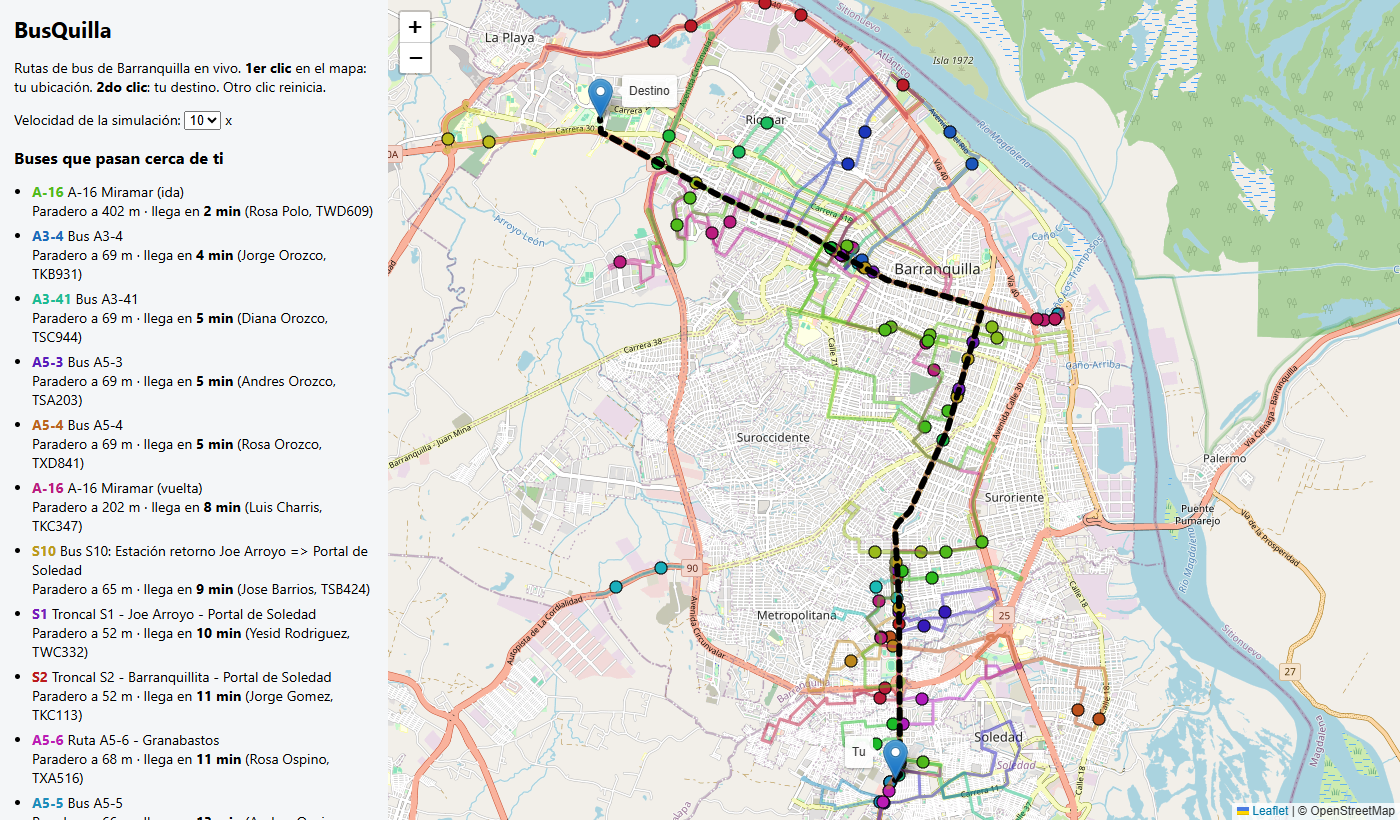
\includegraphics[width=\textwidth]{img/viaje.png}
\caption{BusQuilla con el origen en el Portal de Soledad y el destino en la Universidad del Norte. A la izquierda, rutas cercanas con su ETA y conductor; en el mapa, los buses (círculos de colores) y el viaje recomendado (línea punteada).}\label{fig:app}
\end{figure}

\section{Resultados e interpretación}\label{sec:res}

\subsection{Validación con casos de resultado conocido}
Se construyó la red de juguete de la Figura~\ref{fig:juguete}: la ruta A va de $(0^\circ,0^\circ)$ a $(0^\circ;0{,}02^\circ)$ y la ruta B de $(0^\circ;0{,}02^\circ)$ a $(0{,}02^\circ;0{,}02^\circ)$. Sobre el ecuador, 0,01° equivalen a $6\,371\,000\cdot\pi/18\,000=1\,111{,}95$ m, de modo que cada ruta mide 2\,223,9 m. El viaje óptimo se calcula a mano: esperar el bus A (5 min), recorrerla completa ($2\,223{,}9/333=6{,}678$ min), transbordar (5 min) y recorrer B (6,678 min), para un total de 23,357 minutos. Las cuatro pruebas de la Tabla~\ref{tab:pruebas} se ejecutan con \texttt{node test.js} y todas pasan.

\begin{table}[H]
\centering
\caption{Pruebas automáticas}\label{tab:pruebas}
\begin{tabular}{>{\raggedright\arraybackslash}p{6.4cm}>{\raggedright\arraybackslash}p{6.2cm}l}
\toprule
Caso & Resultado esperado & Estado \\
\midrule
Haversine entre $(0,0)$ y $(1,0)$ & 111\,194,93 m & Pasa \\
Viaje con transbordo en la red de juguete & 23,357 min; tramos A(0$\to$2), B(0$\to$2) & Pasa \\
Destino a 100 m del origen & Caminar, 1,33 min & Pasa \\
ETA: $L=1000$, $u=200$, $v=100$, $c_i=600$ & Ida 4; vuelta 12; cualquiera 4 min & Pasa \\
\bottomrule
\end{tabular}
\end{table}

\subsection{Estructura de la red}
El grafo real tiene $|V|=1\,815$ vértices, 1\,774 aristas de bus y 15\,339 aristas de transbordo, en total $|E|=17\,113$. La suma de grados es $34\,226=2|E|$, como predice el lema del apretón de manos, y el grado promedio es 18,86. La densidad, $|E|/\binom{n}{2}\approx 1{,}04$\,\%, muestra que es un grafo disperso, típico de redes de transporte (Newman, 2018). La distribución de grados es muy desigual (Tabla~\ref{tab:grados}): 519 paraderos tienen grado 1 o 2 (solo los toca su propia ruta), mientras que 321 tienen grado mayor que 25. Los vértices de mayor grado (110) están en la zona de la estación de retorno Joe Arroyo de Transmetro, sobre la Carrera 46, donde coinciden las rutas A9-3, A7-1, A7-3, A7-4, GM, A8-1 y A9-4: es el principal centro de transbordos de la red.

\begin{table}[H]
\centering
\caption{Distribución de grados de los paraderos}\label{tab:grados}
\begin{tabular}{lrr}
\toprule
Grado & Paraderos & Porcentaje \\
\midrule
1--2 & 519 & 28,6\,\% \\
3--10 & 483 & 26,6\,\% \\
11--25 & 492 & 27,1\,\% \\
26 o más & 321 & 17,7\,\% \\
\bottomrule
\end{tabular}
\end{table}

En cuanto a la conectividad, el grafo tiene dos componentes conexas: una gigante de 1\,807 vértices que contiene a 40 de las 41 rutas, y un fragmento de 8 vértices correspondiente a la ruta intermunicipal Baranoa--Barranquilla, cuya relación en OpenStreetMap está incompleta. Esto significa que, con transbordos, prácticamente cualquier paradero de la red puede alcanzarse desde cualquier otro. Si se observa el grafo ``de rutas'' (un vértice por ruta y una arista si dos rutas tienen un transbordo posible), hay 365 pares de rutas conectadas de 820 posibles (densidad 0,45). Las troncales de Transmetro (R1, S1, R10, S10) son las más conectadas, con 38 rutas cada una, seguidas por la A-16 Miramar con 37, lo que confirma su papel de columna vertebral del sistema.

\subsection{Viajes de ejemplo}
La Tabla~\ref{tab:viajes} muestra viajes reales calculados por el programa entre lugares conocidos de la ciudad. En todos los casos el bus reduce el tiempo frente a caminar entre un 58\,\% y un 69\,\%, y en tres de los cuatro casos el mejor viaje combina dos rutas que el usuario podría no conocer.

\begin{table}[H]
\centering
\caption{Viajes recomendados por BusQuilla}\label{tab:viajes}
\begin{tabular}{llrr}
\toprule
Origen $\to$ Destino & Rutas (km en bus) & Bus (min) & A pie (min) \\
\midrule
Portal de Soledad $\to$ Uninorte & R10 (11,9) $\to$ U-30 (5,2) & 65,5 & 181 \\
Paseo Bolívar $\to$ C.C. Buenavista & B2 (3,1) $\to$ A9-3 (3,9) & 33,1 & 78 \\
Estadio Metropolitano $\to$ Gran Malecón & R1 (9,5) $\to$ GM (2,2) & 48,5 & 118 \\
Portal de Soledad $\to$ Joe Arroyo & R1 (11,9) & 40,9 & 130 \\
\bottomrule
\end{tabular}
\end{table}

\subsection{Experimento con viajes aleatorios}
Para medir el aporte de la herramienta de forma más general se generaron 300 pares origen--destino aleatorios dentro del área urbana (semilla fija para que el experimento sea reproducible). El 69,3\,\% de los puntos de la ciudad tiene al menos un paradero a menos de 600 m, y un punto cualquiera tiene en promedio 3,7 rutas cercanas. En 124 de los 300 viajes el bus es mejor que caminar (en los demás, el origen o el destino quedan fuera de la cobertura de las rutas mapeadas o están tan cerca que conviene caminar). De esos 124 viajes, solo 49 (39,5\,\%) se resuelven con una ruta directa; 57 (46,0\,\%) necesitan un transbordo y 18 (14,5\,\%) dos o más. El tiempo promedio de los viajes recomendados fue de 32,9 minutos frente a 52,6 minutos caminando, un ahorro del 37\,\%.

\textbf{Interpretación.} Este resultado es el corazón del argumento de impacto: en seis de cada diez viajes que conviene hacer en bus, la mejor opción requiere combinar rutas. Un usuario que solo conoce ``su'' ruta directa, o que no sabe que puede transbordar, está perdiendo tiempo o directamente no ve una alternativa. A esto se suma la espera: si la frecuencia de una ruta es de 15 a 20 minutos, saber dónde está el bus permite salir de casa en el momento justo en lugar de esperar en promedio la mitad de esa frecuencia en el paradero, que es justamente el beneficio observado en los estudios de información en tiempo real (Watkins et al., 2011; Brakewood y Watkins, 2019).

\subsection{Desempeño}
En un computador portátil común, construir el grafo tarda menos de 0,1 s y cada consulta de Dijkstra tarda en promedio unos 7 ms, por lo que la respuesta al clic es instantánea para el usuario. Esto justifica haber elegido la implementación $O(n^2)$, más simple, en lugar de una con montículo.

\section{Conclusiones y limitaciones}

\subsection{Conclusiones}
\begin{enumerate}
\item La red de buses de Barranquilla se modela de forma natural como un grafo ponderado simple y no dirigido en el que los pesos son tiempos. Separar los paraderos por ruta y representar los transbordos como aristas con costo de espera permite que un solo algoritmo de camino más corto decida a la vez qué rutas tomar, dónde bajarse y dónde transbordar.
\item El algoritmo de Dijkstra resuelve el problema de forma exacta y en milisegundos para la red real de 1\,815 puntos de parada. Las pruebas con resultado conocido validan tanto la distancia de Haversine como el camino mínimo y la fórmula de llegada.
\item La aritmética modular permite describir el movimiento de ida y vuelta de un bus con un único número y deducir una fórmula cerrada para su tiempo de llegada.
\item El análisis estructural muestra una red dispersa pero conexa, con un centro de transbordos claro en la estación Joe Arroyo y con las troncales de Transmetro como rutas más conectadas.
\item El experimento con viajes aleatorios muestra que la mayoría de los viajes óptimos requieren transbordos, lo que respalda la necesidad de una herramienta que muestre ``rutas que también sirven'' además de la posición de los buses.
\end{enumerate}

\subsection{Limitaciones y trabajo futuro}
\begin{itemize}
\item \textbf{Posiciones simuladas.} La ubicación de los buses y los conductores son simulados, pues no hay datos GPS públicos. El modelo está diseñado para que, si las empresas publicaran sus posiciones (por ejemplo en formato GTFS Realtime), bastara con reemplazar la variable $u$ de cada bus por el dato real.
\item \textbf{Cobertura de datos.} OpenStreetMap contiene principalmente las rutas de Transmetro y pocas rutas del transporte colectivo tradicional, que es justamente el más usado. Mapear más rutas, por ejemplo con ayuda de los mismos usuarios, aumentaría la cobertura del 69\,\% actual.
\item \textbf{Simplificaciones del modelo.} Velocidad constante (sin congestión por hora del día), espera fija de 5 minutos en el cálculo del viaje, rutas recorridas en ambos sentidos y rutas circulares tratadas como ida y vuelta. Un modelo más fiel usaría un grafo dirigido y pesos dependientes del tiempo.
\item \textbf{Alcance.} Es una versión alpha pensada para computador; no incluye tarifas, horarios de operación ni accesibilidad para personas con movilidad reducida.
\end{itemize}

\section*{Referencias}
\begin{list}{}{\setlength{\leftmargin}{1.27cm}\setlength{\itemindent}{-1.27cm}\setlength{\itemsep}{4pt}}
\item Agafonkin, V. (2023). \textit{Leaflet} (versión 1.9.4) [Software]. \url{https://leafletjs.com}
\item Brakewood, C., y Watkins, K. (2019). A literature review of the passenger benefits of real-time transit information. \textit{Transport Reviews, 39}(3), 327--356. \url{https://doi.org/10.1080/01441647.2018.1472147}
\item Contexto. (2023). \textit{Siete datos de la encuesta de Barranquilla Cómo Vamos para tomarle el pulso a la ciudad}. \url{https://contextomedia.com/siete-datos-de-la-encuesta-de-barranquilla-como-vamos-para-tomarle-el-pulso-a-la-ciudad/}
\item Contexto. (2024). \textit{Más seguridad y mayor participación ciudadana, las demandas de los barranquilleros en la nueva encuesta de Barranquilla Cómo Vamos}. \url{https://contextomedia.com/mas-seguridad-y-mayor-participacion-ciudadana-las-demandas-de-los-barranquilleros-en-la-nueva-encuesta-de-barranquilla-como-vamos/}
\item Cormen, T. H., Leiserson, C. E., Rivest, R. L., y Stein, C. (2022). \textit{Introduction to algorithms} (4.\textsuperscript{a} ed.). MIT Press.
\item Dijkstra, E. W. (1959). A note on two problems in connexion with graphs. \textit{Numerische Mathematik, 1}, 269--271. \url{https://doi.org/10.1007/BF01386390}
\item El País. (2024, 20 de febrero). \textit{Pasaje en Barranquilla: la tarifa del Transmetro y los descuentos a estudiantes en 2024}. \url{https://elpais.com/america-colombia/2024-02-20/pasaje-en-barranquilla-la-tarifa-del-transmetro-y-los-descuentos-a-estudiantes-en-2024.html}
\item Ferris, B., Watkins, K., y Borning, A. (2010). OneBusAway: Results from providing real-time arrival information for public transit. En \textit{Proceedings of the SIGCHI Conference on Human Factors in Computing Systems} (pp. 1807--1816). ACM. \url{https://doi.org/10.1145/1753326.1753597}
\item Gobernación del Atlántico. (2025). \textit{Anuario estadístico del Atlántico 2024. Capítulo 2: Demografía}. \url{https://www.atlantico.gov.co/images/stories/adjuntos/planeacion/anuarios/anuario2024/anuario2024_capitulo2_demografia.pdf}
\item La Silla Vacía. (2023). \textit{Detector: Transmetro sí moviliza menos pasajeros de los que proyectó}. \url{https://www.lasillavacia.com/detector-de-mentiras/debatible/detector-transmetro-si-moviliza-menos-pasajeros-de-los-que-proyecto/}
\item Newman, M. (2018). \textit{Networks} (2.\textsuperscript{a} ed.). Oxford University Press.
\item OpenStreetMap contributors. (2026). \textit{OpenStreetMap: relaciones de rutas de bus del Área Metropolitana de Barranquilla} [Base de datos, licencia ODbL]. \url{https://www.openstreetmap.org}
\item Overpass API. (2026). \textit{Overpass API} [Software]. \url{https://overpass-api.de}
\item Rosen, K. H. (2019). \textit{Discrete mathematics and its applications} (8.\textsuperscript{a} ed.). McGraw-Hill Education.
\item Sinnott, R. W. (1984). Virtues of the haversine. \textit{Sky and Telescope, 68}(2), 159.
\item Watkins, K. E., Ferris, B., Borning, A., Rutherford, G. S., y Layton, D. (2011). Where is my bus? Impact of mobile real-time information on the perceived and actual wait time of transit riders. \textit{Transportation Research Part A: Policy and Practice, 45}(8), 839--848. \url{https://doi.org/10.1016/j.tra.2011.06.010}
\end{list}

\end{document}
